\documentclass{article}
\usepackage[english]{babel}
\usepackage[letterpaper,top=2cm,bottom=2cm,left=2.5cm,right=2.5cm,marginparwidth=1.25cm]{geometry}

\usepackage[leqno]{amsmath}
\usepackage{enumitem, nccmath,lipsum,amssymb,xcolor,xparse,listings, blindtext,array, hyperref}
\usepackage[most]{tcolorbox}

\NewDocumentCommand{\codeword}{v}{
\texttt{\textcolor{blue}{#1}}
}

\lstset{language=C, keywordstyle={\bfseries \color{blue}}}

\NewDocumentCommand{\mynote}{+O{}+m}{%
  \begingroup
  \tcbset{%
    noteshift/.store in=\mynote@shift,
    noteshift=1.5cm
  }
  \begin{tcolorbox}[nobeforeafter,
    enhanced,
    sharp corners,
    toprule=0.5pt,
    bottomrule=0.5pt,
    leftrule=0pt,
    rightrule=0pt,
    colback=green!10,
    #1,
    left skip=\mynote@shift,
    right skip=\mynote@shift,
    overlay={\node[right] (mynotenode) at ([xshift=-\mynote@shift]frame.west) {\textbf{Note:}} ;},
    ]
    #2
  \end{tcolorbox}
  \endgroup
  }
\makeatother

\newcommand{\mytext}[1]% #1 = same as intertext
{&\parbox{0.9\textwidth}{\rule{0pt}{.5\baselineskip}\\
\textrm{#1}\\
\rule{0pt}{.5\baselineskip}}&\\}

\newcounter{exercise}
\newcounter{problem}[exercise]
\newcommand{\myitem}{\stepcounter{problem}\tag*{\alph{problem})}}

\title{Introduction to Artificial Intelligence: Assignment 2.}
\author{Mashenkov Timofei B23-ISE-05 \\ \href{mailto:t.mashenkov@innopolis.university}{t.mashenkov@innopolis.university}}
\begin{document}
\maketitle{}

\section{Evolutionary Algorithm}

\subsection{Flow}

\begin{enumerate}
  \item \textit{Initialization:} Generate an initial population of chromosomes.
  \item \textit{Selection:} Sort the population based on fitness and select the top-performing chromosomes.
  \item \textit{Crossover:} Combine the selected chromosomes to create new offspring.
  \item \textit{Mutation:} Introduce random changes in the offspring to maintain diversity.
  \item \textit{Replacement:} Replace the least fit chromosomes with the new offspring.
  \item \textit{Termination:} Repeat steps 2-5 until a stopping criterion is met (solution with 0 fitness value is found).
\end{enumerate}

\subsection{Algorithm Overview}

The evolutionary algorithm (EA) consists of the following components, they have been tested for a long time,
so the ranges of values that were used in testing are given:

\begin{itemize}
    \item \textbf{Population Size:} 2000 chromosomes (sudoku tables).
    \item \textbf{Mutation Rate:} 3-90\%.
    \item \textbf{Generations:} 500–2000 generations.
    \item \textbf{Stagnation Threshold:} 40–100 generations without improvement.
\end{itemize}

\subsection{Initial Population}

The initial population is generated by filling the undefined cells (hyphens) with random numbers in available (remain
after removing predefined) range of numbers, ensuring that the predefined numbers remain unchanged.

\subsection{Fitness Function}

The fitness function evaluates the quality of a chromosome. Since numbers in rows are unique, the fitness is determined
by counting the number of duplicates in columns and subgrids:

\[
\text{Fitness} = \text{Number of Column Duplicates} + \text{Number of Subgrid Duplicates}
\]

A perfect solution has a fitness value of 0.

\subsection{Crossover Operation}

Crossover combines two parent chromosomes by selecting the best elements from each parent to create a new offspring. The selection is based on the local fitness of each cell.

\subsection{Mutation Operation}

Mutation introduces random changes in the chromosome to maintain diversity in the population. It swaps two random cells in a row, provided they are not predefined.

\subsection{Selection Process}

The selection process involves sorting the population based on fitness and choosing the top-performing chromosomes for the next generation. The population is replenished with new chromosomes generated from the best solutions.

\section{Experimental Setup}

The algorithm was tested on Sudoku puzzles with varying numbers of givens (20 to 40). For each number of givens, at least 10 tests were conducted. The performance was measured in terms of average and maximum fitness values over the final generations.

\section{Results}

The algorithm successfully solved Sudoku puzzles across different complexity levels. The plots in References section
show the average fitness, maximum fitness and average time for each complexity level. 

\begin{itemize}
    \item \textbf{Easy Difficulty:}  
      \begin{itemize}
        \item average time 3.6205454545454545
        \item maximum fitness 55.45454545454545
        \item average fitness 22.845454545454544
      \end{itemize}
  \item \textbf{Medium Difficulty:}  
    \begin{itemize}
      \item average time 6.5760000000000005
      \item maximum fitness 61.25
      \item average fitness 25.15
    \end{itemize}
  \item \textbf{Hard Difficulty:}
    \begin{itemize}
      \item average time 6.489999999999999
      \item maximum fitness 63.266666666666666
      \item average fitness 26.283333333333335
    \end{itemize}
\end{itemize}

\section{Conclusion}

The evolutionary algorithm effectively solves Sudoku puzzles by iteratively improving the population of candidate solutions. The results demonstrate the algorithm's capability to handle puzzles of varying difficulty levels. Future work could explore more sophisticated mutation and crossover operators to enhance convergence speed.

\section{References}

\begin{thebibliography}{99}
    \bibitem{classification}
    \href{Sudoku Complexity Classification.}{https://sudoku2.com/sudoku-tips/how-sudoku-difficulty-is-measured/}, 2023.
\end{thebibliography}

\begin{figure}[h]
    \centering
   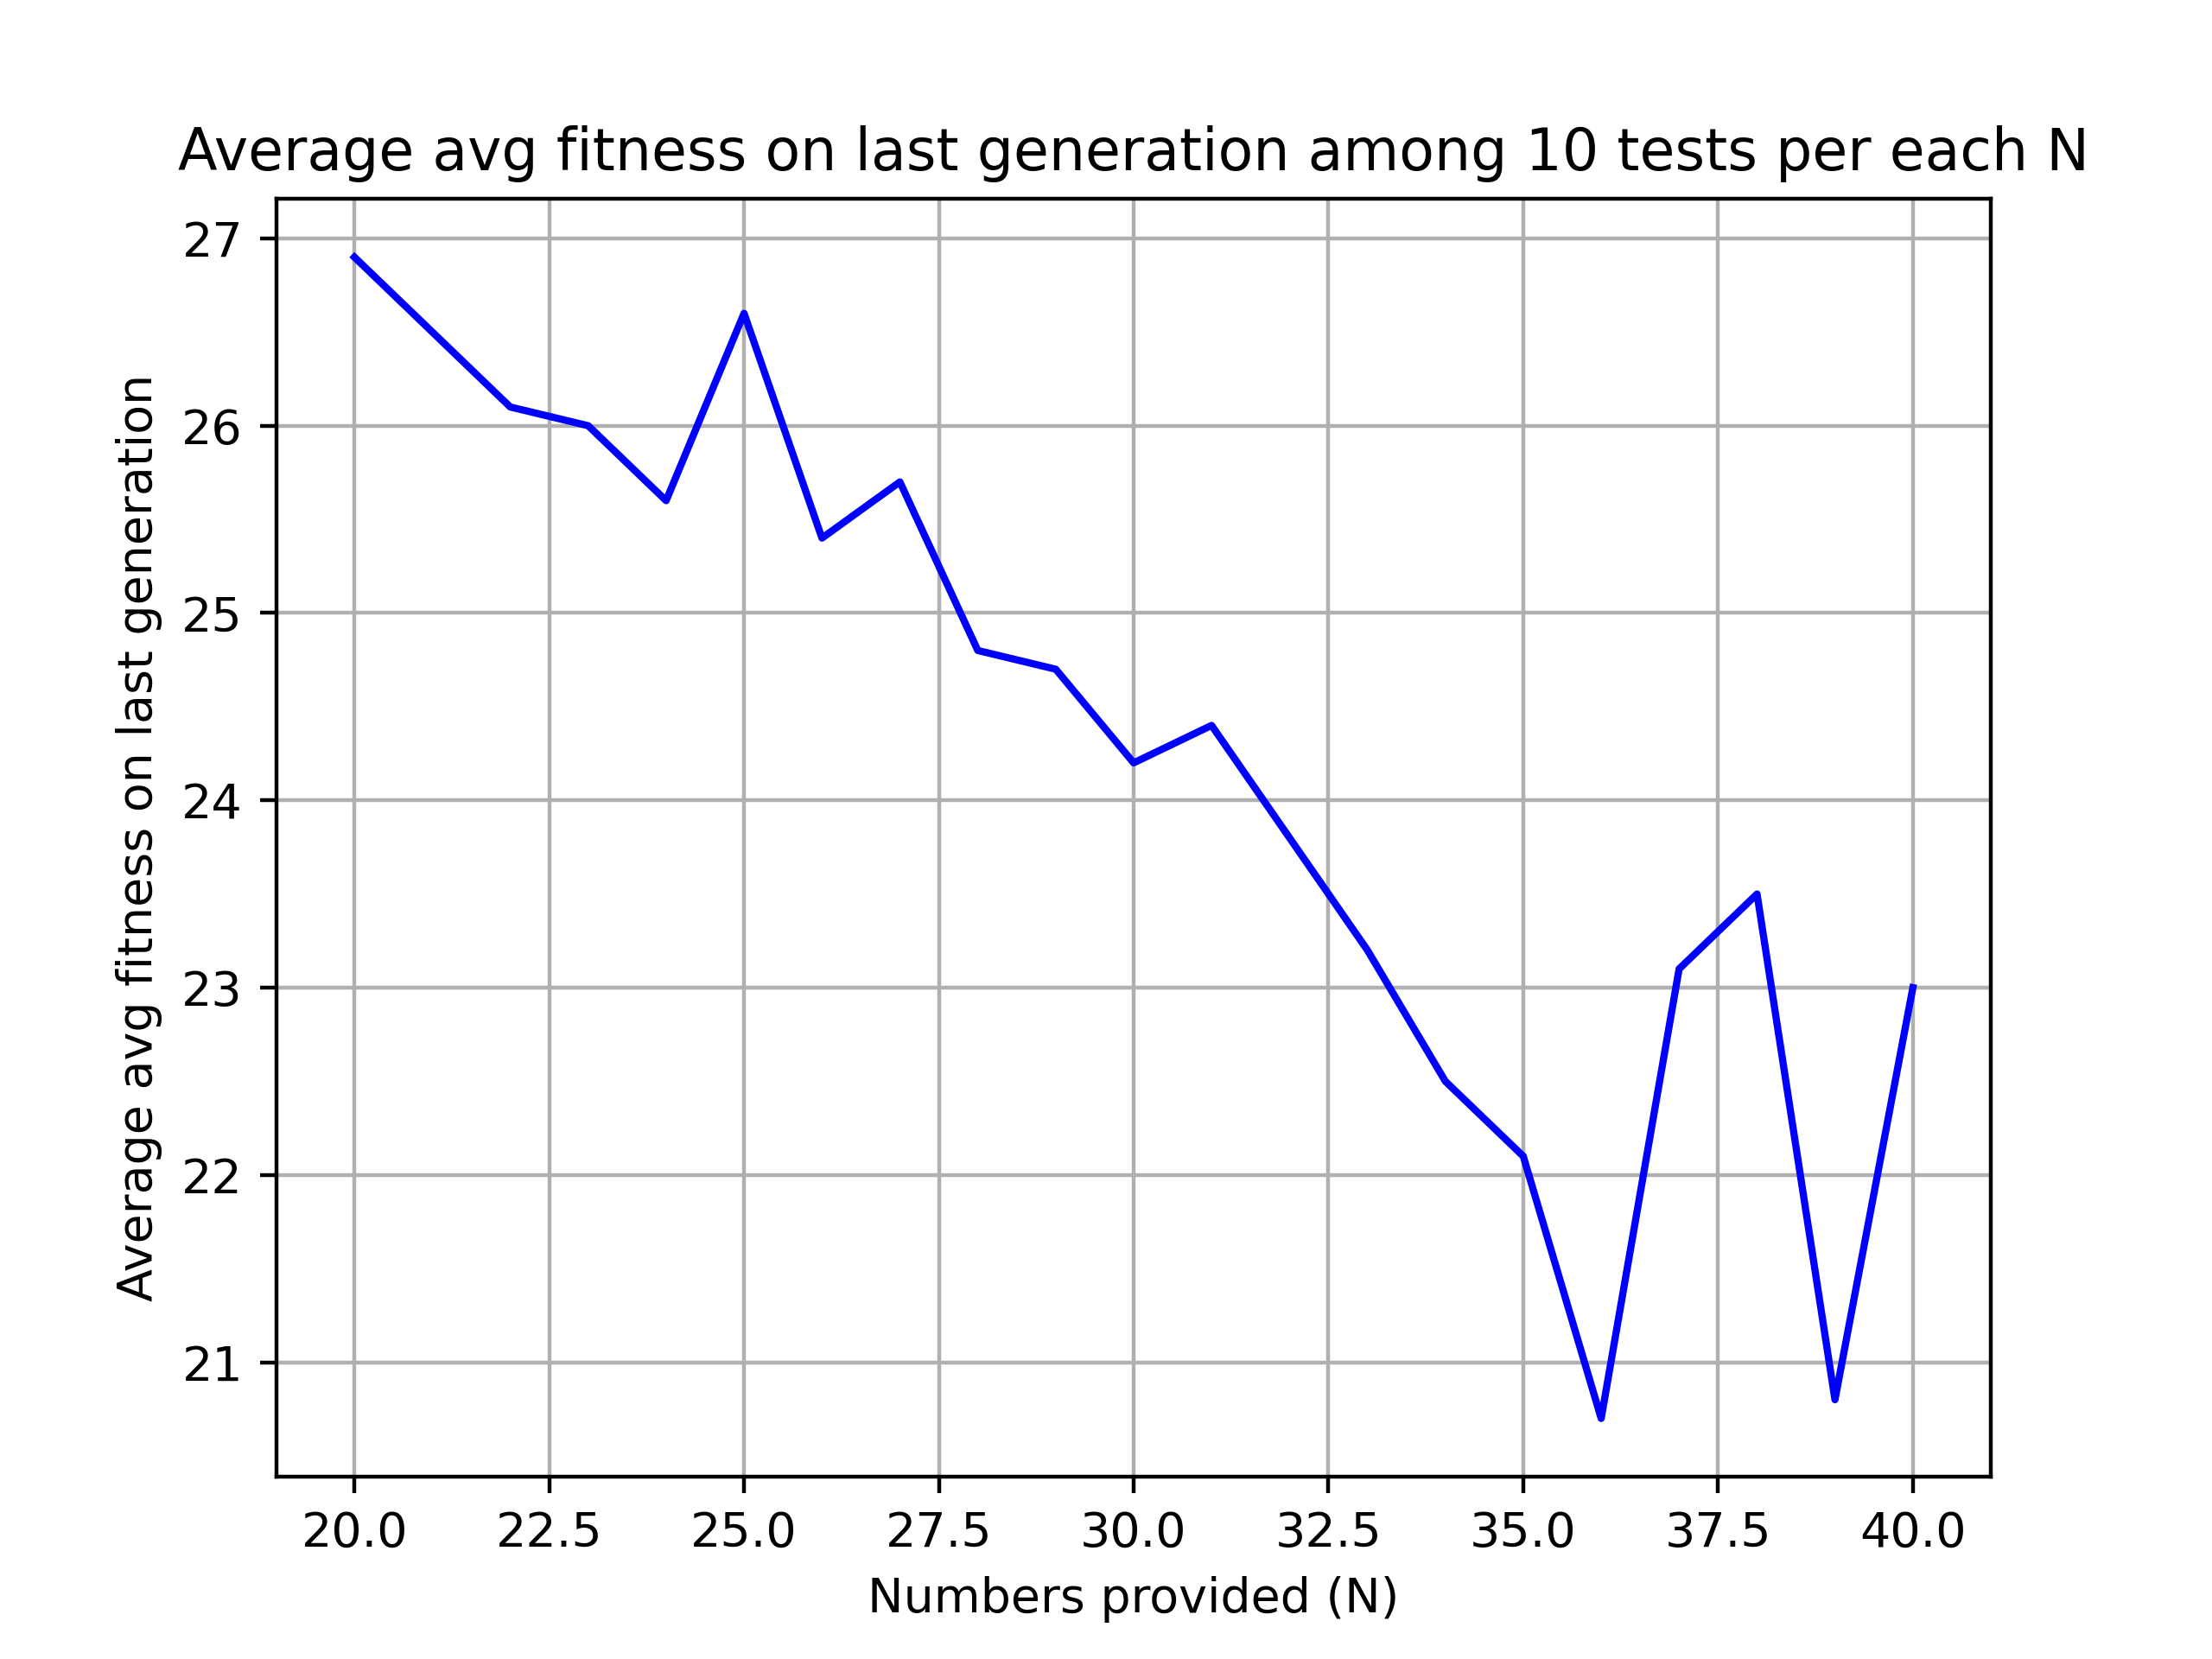
\includegraphics[width=0.8\linewidth]{avgfit.png}
    \caption{Average fitness.}
\end{figure}
\begin{figure}[h]
    \centering
   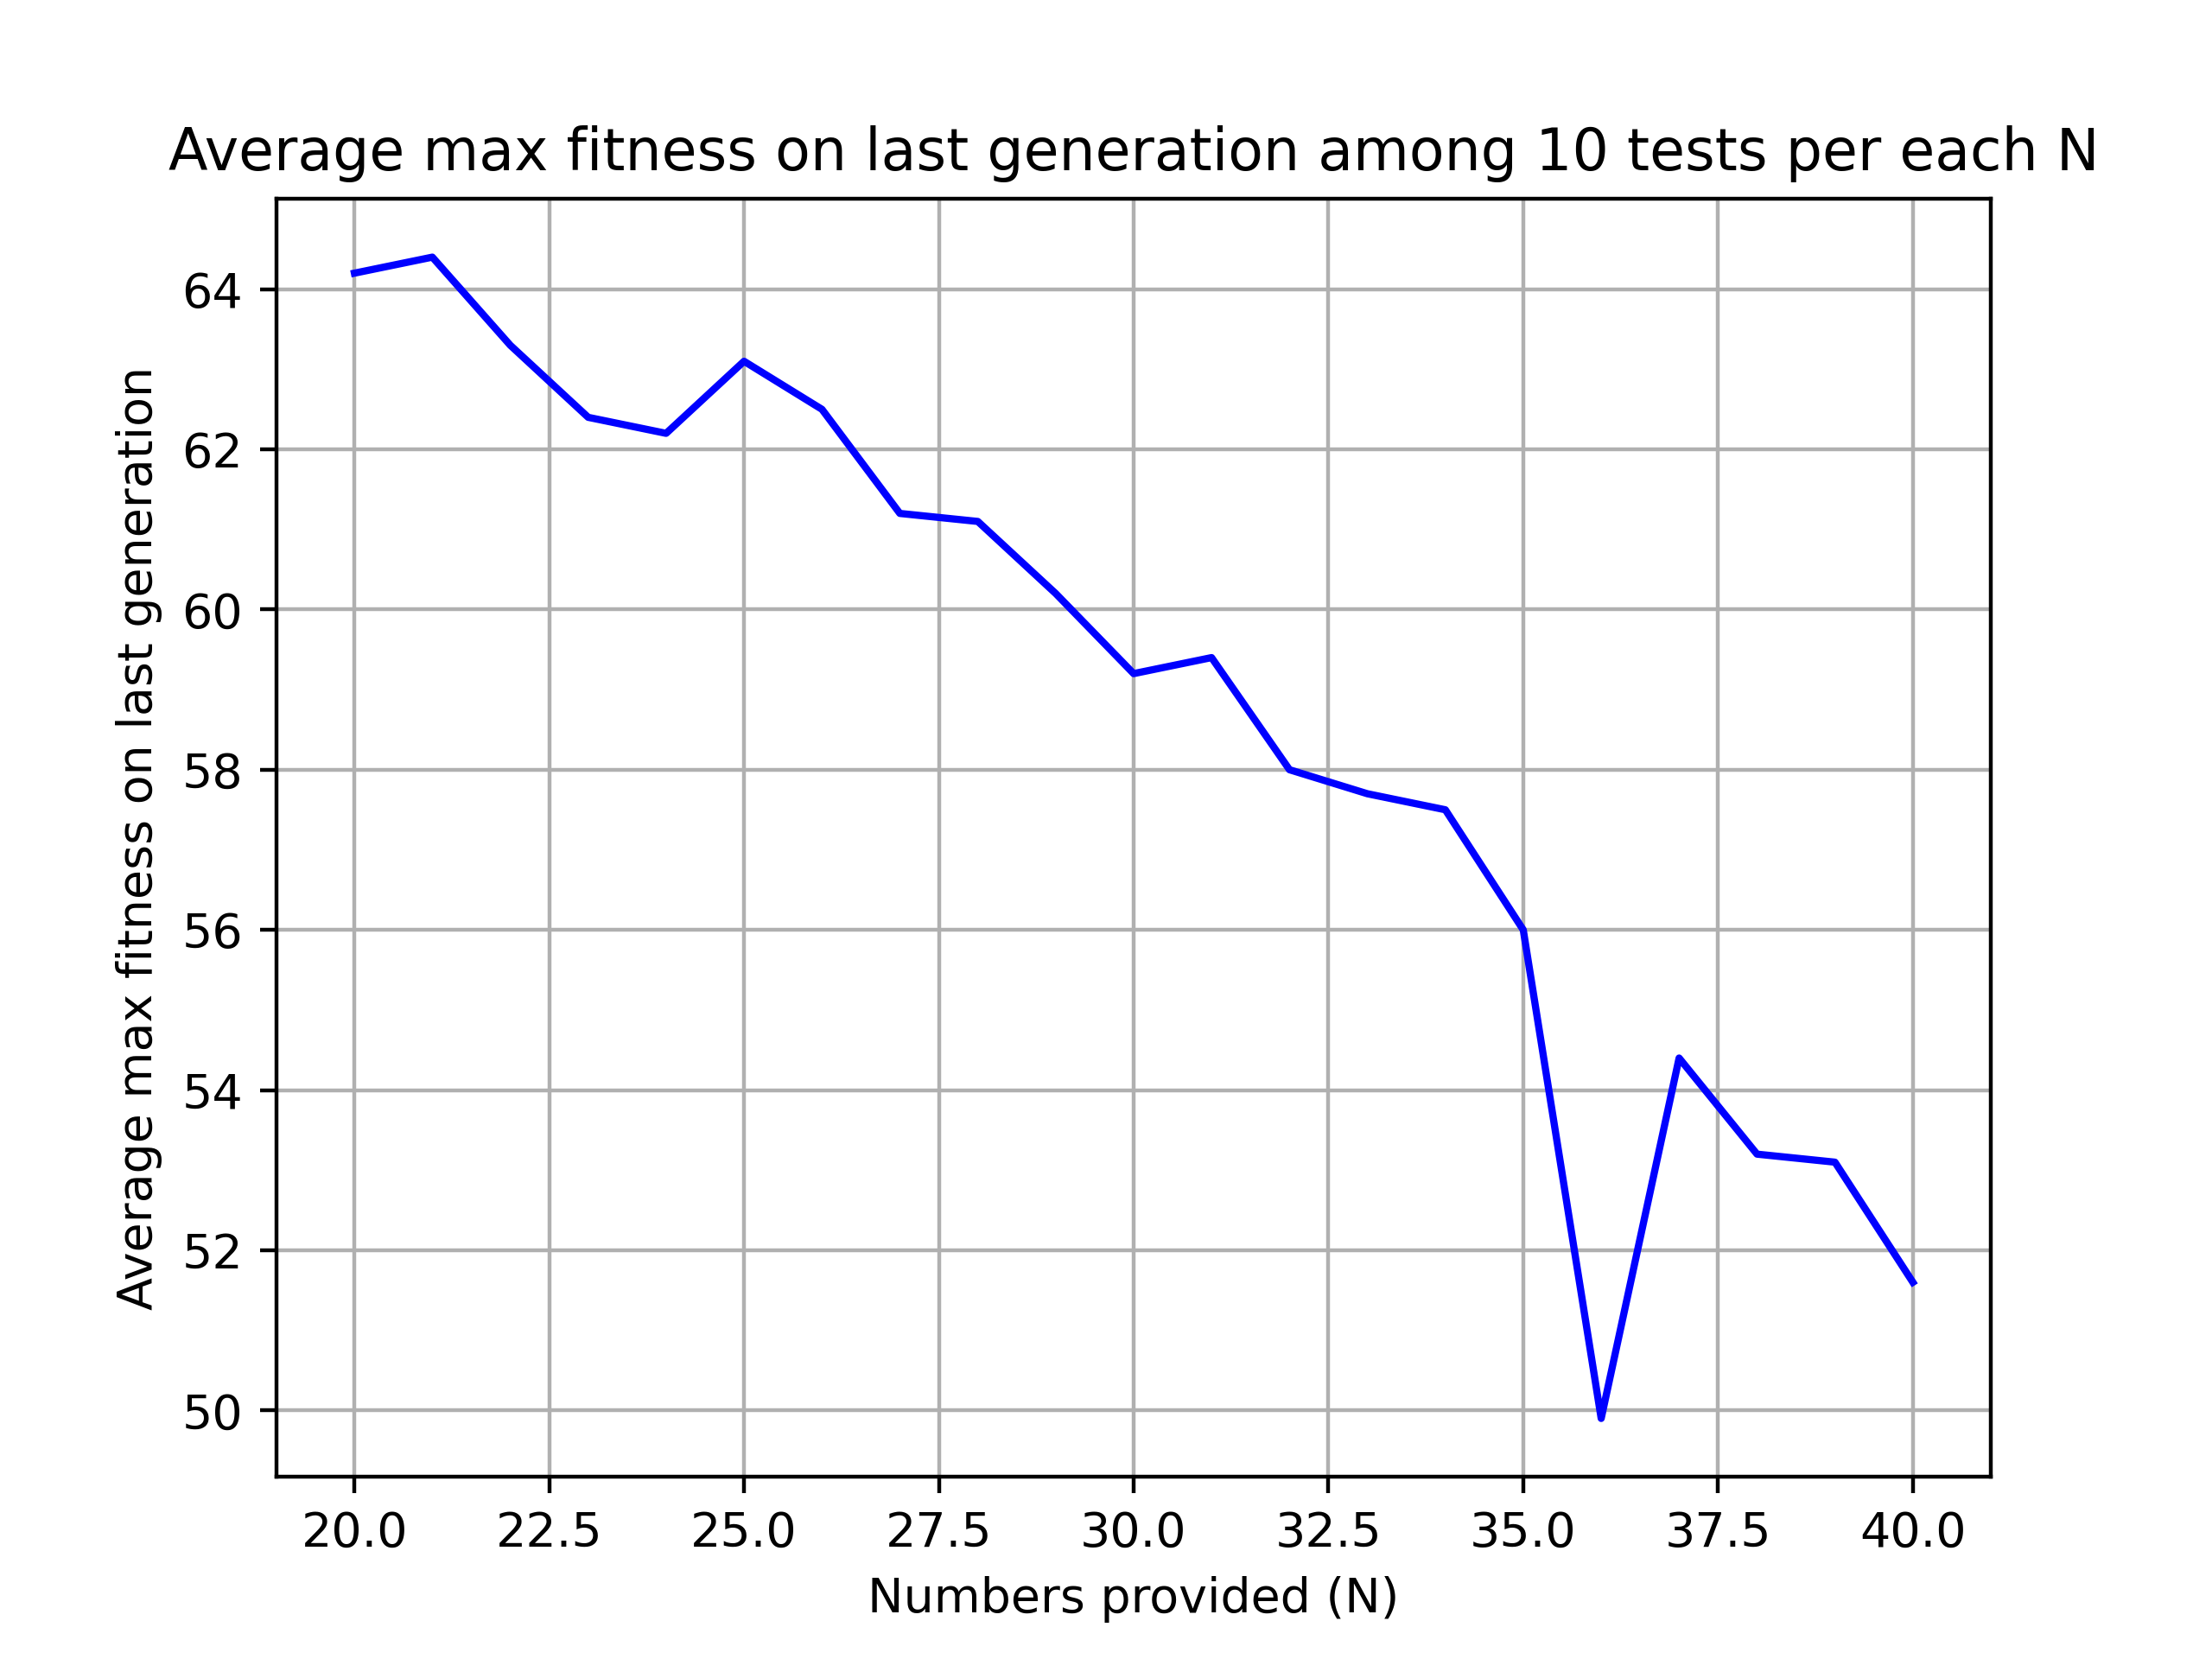
\includegraphics[width=0.8\linewidth]{maxfit.png}
    \caption{Maximum fitness.}
\end{figure}
\begin{figure}[h]
    \centering
   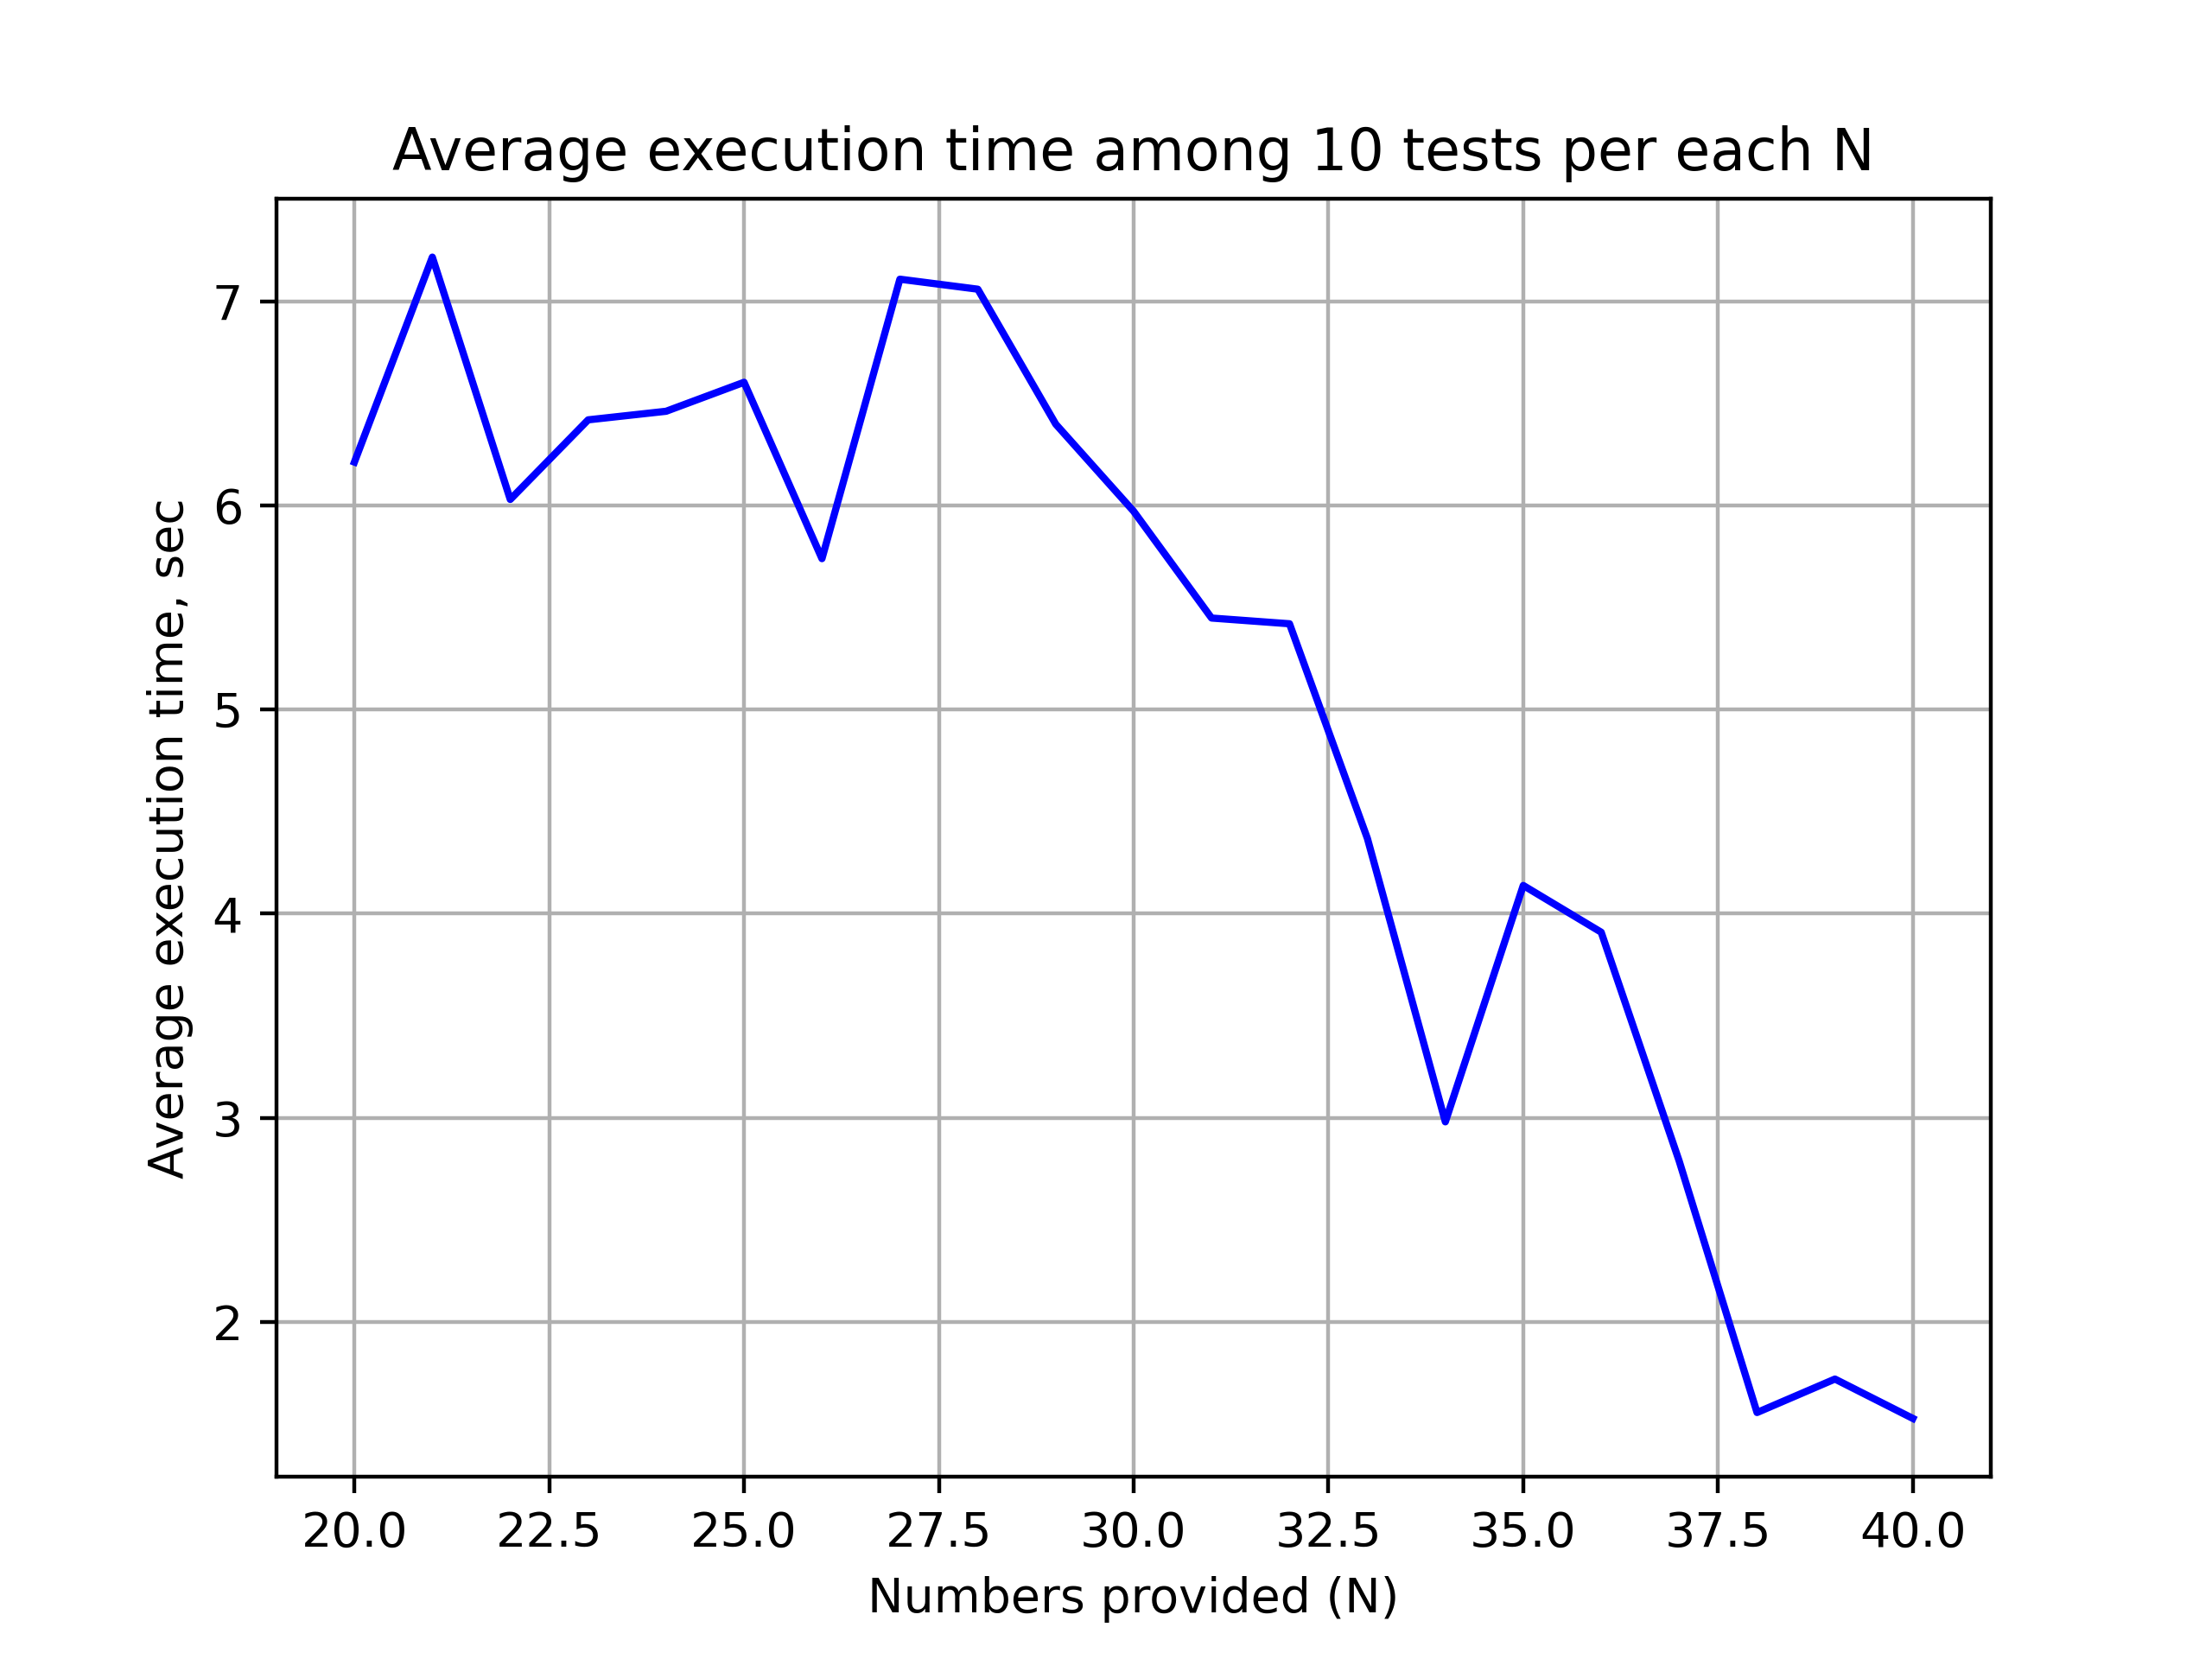
\includegraphics[width=0.8\linewidth]{exec.png}
    \caption{Execution time.}
\end{figure}

\end{document}
